\section{Process}
Waiting for more text to fill...
\subsection{Overall}
Overall technical route
In order to obtain a smaller model, less training and running with better performance, we decided to make multiple models and training improvements based on DCGAN [2] and improve it through multiple sets of experiments.
Figure 0 is the overall technical roadmap for this study.

% 
\begin{center}
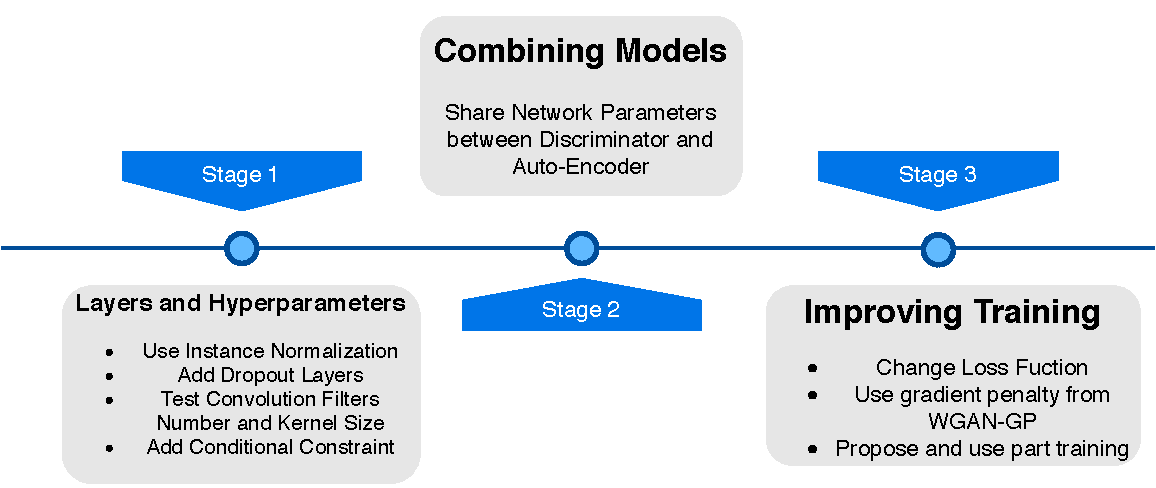
\includegraphics[width=0.5\textwidth]{figures/roadmap.pdf}
\end{center}

\subsection{Research Process}

\subsection{Model Overview}

After the above research, we finally obtained the conditional facial image generation and adjustment model based on GAN\upcite{gan},
    which is a method of facial image generation and adjustment using machine learning (as shown in Figure 1).

The model consists of a generative confrontation network and a self-encoding network.
The main components in the network are the encoder and the decoder and the two networks share the network parameters of the encoder.
In this model, the generator generates a facial image from the noise and face attribute conditions and then combines the original image with the new face attribute condition to obtain a new image by adjusting the network.


\subsection{Decoder and Encoder}

The main component encoder and decoder are used for the conversion of feature vectors and images.
An encoder is used to extract features from an image.
Using a convolution method, starting from an image of 128 × 128 × 3 (height × width × channel number),
    the convolution operation with step size is continuously performed to extract features while reducing the image dimension.
After each convolution operation, normalization, activation,
    and Dropout\upcite{dropout} are performed in order to extract features from the image as a whole to the local.

The convolutional layer uses a convolution kernel size of 5×5.
The filter is incremented from the 16th layer and the step size is set to 2 so the image dimension is reduced when the feature is extracted,
    and the network is lowered with lower calculation amount.
Since the gradient penalty proposed in WGAN-GP\upcite{wgan-gp} is used in the training,
    our normalization layer chose Instance Normalization\upcite{instance}.
To preserve the image for more information, the activation function uses Leaky ReLU with alpha=0.2.
In order to alleviate the occurrence of over-fitting,
    Dropout\upcite{dropout} is used in the training to randomly hide some neurons to reduce the interaction between filters.

The decoder is used to generate an image from the feature vector.
Using the method of transposition convolution, the same number of filters,
    step size, and convolution kernel are symmetrically used with the encoder.
Normalization and activation are performed after each transposition convolution operation.
The normalization layer and the activation function are normalized to the same instance as the encoder and the Leaky ReLU with alpha = 0.2.


\subsection{Generative Adversial Network}

In generative adversarial networks, the model consists of a fully connected layer and a decoder.
The facial attribute condition is combined with random noise to generate an image by transposing convolution.
The discriminator consists of an encoder and a fully connected layer at the bottom,
    and extracts features by convolution and combines them.
The condition determines whether the image comes from the real world and extracts the facial attribute information implied by the image.

The top of the generator is a fully connected network that joins the input facial attribute conditions and the noise (implicit vector) that conform to the normal distribution into a 4×4×n layer feature map.
After the second and fourth convolution, the feature map connected by the facial attribute condition parameter is added,
    and then the image is generated from the global to the local by the decoder layer by layer.
Finally a convolution operation with a step size of 1 and a filter number of 3 is performed and used.
The tanh function is activated to obtain a three-channel color image of 128 × 128 × 3 size.

The top of the discriminator is an encoder that extracts the feature vector of 4 × 4 × n size from the input image.
Finally, the feature vectors are fully connected.
On the one hand, the vector is connected to the dimension 1.
The Sigmoid activation function is used to normalize the result to 0~1,
    which indicates the possibility that the image comes from real data.
On the other hand, connected to the same dimension as the feature vector,
    the latent facial attribute information is extracted,
    and the result is also normalized to 0~1 using the Sigmoid activation function,
    thereby indicating the possibility that the image has these facial attributes.

For the discriminator loss, since the Sigmoid is used to activate the output,
    in order to ensure that the neuron parameters in the network layer are not too large or too small leading to model out of balance,
    we limit the loss of the discriminator output to 0.02~0.98.
Since the discriminator not only outputs whether the image is from the real world but also contains the facial attribute information implied by the image,
    it includes the GAN loss and the conditional judgment loss.
We expect the discriminator to be as close as possible to the true image discrimination result as close as 0.98,
    and the discriminant result from the generator image is as close as possible to 0.02.
Similarly, it is desirable that the facial attribute information output by the discriminator is as consistent as possible with the real data.
Equation 1, Equation 2, and Equation 3 are the GAN loss and conditional judgment loss of the discriminator, respectively.

\subsection{Auto-Encoder Network}

\subsection{Model Training}